\documentclass{article}

\usepackage{amsmath, amsthm, amssymb}
\usepackage{tikz}
\usepackage{float}

\newtheorem{defn}{Defintion}[section]
\newtheorem{thm}{Theorem}[section]
\newtheorem{cor}[thm]{Corollary}
\newtheorem{lem}[thm]{Lemma}

\title{..}
\author{Edward O'Callaghan}

\begin{document}
\maketitle

\section{Hilbert Space $L^2$}

In the special and unique case of fixed $p=2$ in $L^2(\mathbb{R})$ we obtain a Hilbert
space. Hilbert space $L^2(a,b)$ has the fruitful property that polynomials over
it form a dense subspace.

Let us define the Banach space $L^p(\mathbb{R})\, \forall p \in [1, \infty[$ and then
restrict ourselves to the case of $p=2$ to define the space:
\[
 L^2(\mathbb{R}) = \left\{ f : \mathbb{R} \rightarrow \mathbb{C} : \int_{-\infty}^{\infty} \left| f(x) \right|^2 dx < \infty \right\}.
\]
Herein we show that this space can indeed be equipped with an inner product.

\begin{thm}
The vector space $L^2(\mathbb{R})$ is a Hilbert space with respect to the inner product:
  \[
    \langle f,g \rangle = \int_{-\infty}^{\infty} f(x) \overline{g(x)} \, dx, \, f,g \in L^2(\mathbb{R}).
  \]
\end{thm}

\begin{proof}
We know that, for each $p\in[1,\infty[$, the expression
  \[
    \|f\|_p = \left( \int_{-\infty}^{\infty} |f(x)|^p \, dx \right)^{1/p}
  \]
defines a norm on $L^p(\mathbb{R})$ that makes $L^p(\mathbb{R})$ a Banach
space, and so the special case of $p=2$ it trivially follows $L^2(\mathbb{R})$
is Banach.

The integral in the inner product is well defined when the map $x \mapsto f(x)
\overline{g(x)}$. is within $L^1(\mathbb{R})$ and hence we are required to prove
this. By using Holder's inequality, fixing $p=q=2$, we observe $\forall f,g \in
L^2(\mathbb{R})$ that,
\[
  \int_{-\infty}^{\infty} |f(x) \overline{g(x)}| \, dx \leq
  \left( \int_{-\infty}^{\infty} |f(x)|^2 \, dx \right)^{1/2}
  \left( \int_{-\infty}^{\infty} |g(x)|^2 \, dx \right)^{1/2} < \infty
\]
and so the required results immediately follow.
\end{proof}

\subsection{Linear Operators on $L^2(\mathbb{R})$}

\begin{defn}
We may define three classes of linear operators on $L^2(\mathbb{R})$:
\begin{enumerate}
\item For $a\in\mathbb{R}$, the operator $T_a$, called \textbf{translation} by
      $a$, is defined by \[(T_a f)(x) = f(x-a), x\in\mathbb{R}\].
\item For $b\in\mathbb{R}$, the operator $M_b$, called \textbf{modulation} by
      $b$, is defined by \[(M_b f)(x) = e^{2\pi i b x} f(x), x\in\mathbb{R}\].
\item For $c>0$, the operator $D_c$, called \textbf{dilation} by $c$, is defined
      by \[(D_c f)(x) = \frac{1}{\sqrt{c}} f(x/c), x\in\mathbb{R}\].
\end{enumerate}
\end{defn}

\begin{lem}
The operators $T_a,M_b,D_c : L^2(\mathbb{R}) \to L^2(\mathbb{R})$ are unitary
linear operators in which the following relations hold:
\begin{enumerate}
\item $T_a^{-1} = T_{-a} = (T_a)^{*}$,
\item $M_b^{-1} = M_{-b} = (M_b)^{*}$,
\item $D_c^{-1} = D_{1/c} = (D_c)^{*}$.
\end{enumerate}
\end{lem}

\begin{proof}
easy, you do it!
\end{proof}

\subsection{The $L^2(a,b)$ subspace}

Let us consider the restricted case of squarely integrable functions defined on
the subinterval $S=]a,b[\subseteq\mathbb{R}$ by defining the following space:

\[
  L^2(a,b) = \left\{ f : S \to \mathbb{C} : \int_S |f(x)|^2 \, dx < \infty \right\}.
\]

Following that of the case of $L^2(\mathbb{R})$ one can prove that the subspace
$L^2(a,b)$ is also a Hilbert space equipped with the usual inner product
restricted in domain. The associated induced norm is then:

\[
  \|f\|_{L^2(a,b)} = \sqrt{\int_S |f(x)|^2 \, dx}, f \in L^2(a,b).
\]

Now recall that, for each $p\in[1,\infty[$, the vector space $C_c(\mathbb{R})$
is a dense subspace of $L^p(\mathbb{R})$. Hence, by considering
$S$ as a finite interval we see that continoues functions with
the compact support of $S$ are then dense in $L^2(a,b)$.

\begin{thm}
  The set of polynomials on $]a,b[\subseteq\mathbb{R}$ is dense in $L^2(a,b)$.
\end{thm}

\begin{proof}
We are required to prove that, for each $f\in L^2(a,b)$ and each $\epsilon >0$
we can find a polynomial $\mathcal{P}$ such that:

\[
  \| f - \mathcal{P} \|_{L^2(a,b)} = \left( \int_a^b | f(x) - \mathcal{P}(x) |^2 \, dx \right)^{1/2} \leq \epsilon.
\]

Note that we may extend any function $f \in L^2(a,b)$ to $f \in L^2(a,b)$ by
fixing $f(x)=0$ for any $x \notin [a,b]$. Now recall that we can find a
function $g \in C_c(\mathbb{R})$ such that $\| f  - g \|_{L^2(\mathbb{R})} \leq
\epsilon /2$. This implies the following:

\begin{align*}
  \| f - g \|_{L^2(a,b)} &= \sqrt{\int_a^b | f(x) - g(x) |^2 \, dx}
  \\ &\leq \sqrt{\int_{-\infty}^{\infty} | f(x) - g(x) |^2 \, dx}
  \\ &\leq \epsilon /2.
\end{align*}

The restriction of $g |_{[a,b]}$ is continuous and so we know there exists a
polynomial $\mathcal{P}$ such that:

\begin{align*}
  | g(x) - \mathcal{P}(x) | &\leq \frac{\epsilon}{2\sqrt{b-a}}, \, \forall x \in [a,b].
  \intertext{Given some choose of $\mathcal{P}$ implies that}
  \| g - \mathcal{P} \|_{L^2(a,b)} &= \sqrt{\int_a^b | g(x) - \mathcal{P}(x) |^2 \, dx}
  \\ &= \sqrt{\int_a^b \left( \frac{\epsilon}{2\sqrt{b-a}} \right)^2 \, dx}
  \\ &\leq \epsilon /2.
\end{align*}

Combining these results we obtain the following:

\begin{align*}
  \| f - \mathcal{P} \|_{L^2(a,b)} &= \| (f-g) + (g-\mathcal{P}) \|_{L^2(a,b)}
  \\ &\leq \| f - g \|_{L^2(a,b)} + \| g - \mathcal{P} \|_{L^2(a,b)}
  \\ &\leq \epsilon.
\end{align*}

\end{proof}

\subsection{Fourier Series}

The Fourier series is a way to express certain functions with particular
properties in terms of a power series of trigonometric functions. More
generally, the series is a generator function for which sinusoids and
co-sinusoids form the orthonormal basis. The quintessential property is that of
periodicity for which we make precise here:

\begin{defn}
  A function $f$ defined over the reals is said to be a \emph{periodic
  function} with period $2\pi$ iff, $f(x + 2\pi) = f(x), \forall x \in \mathbb{R}$.
\end{defn}

Naturally we may then consider functions $f \in L^2(-\pi,\pi)$ as periodic
functions with period $2\pi$. Recall that $L^2(-\pi,\pi)$ is a Hilbert space
equipped with the inner product

\[
  \langle f,g \rangle = \int_{-\pi}^{\pi} f(x) \overline{g(x)} \, dx,
  \,\, f,g \in L^2(-\pi,\pi).
\]

Formally we may now define the Fourier series in the complex form as follows:

\begin{defn}
  \[
    f \sim \sum_{k=-\infty}^{\infty} c_k e^{ikx};
  \]
  where the coefficients $c_k$ are given by the integral transform:
  \[
    c_k = \frac{1}{2\pi} \int_{-\pi}^{\pi} f(x) e^{-ikx} \, dx.
  \]
\end{defn}

Intuitively we can think of the Fourier series as the decomposition of a given
function $f$ into harmonic components with representative frequencies $k/2\pi,
k\in\mathbb{N}$ for each of the sine and cosine spanning basis. Here, the
magnitude of contribution at each of these frequencies is given by the Fourier
coefficient $c_k$, which is in fact the Fourier transform.  The following
illustration demonstrates this decomposition intuition graphically.

\begin{figure}[H]
\centering
\caption{Illustration of a Fourier decomposition of $sinc(x)$.}
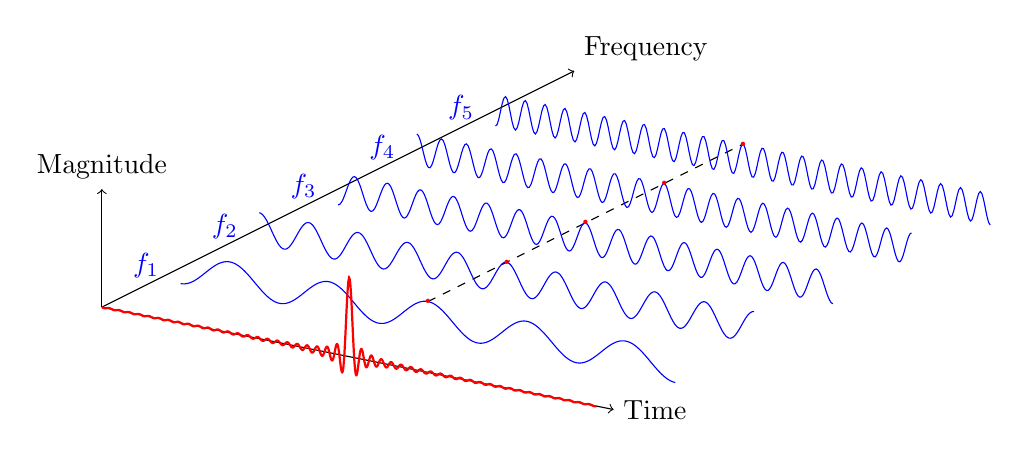
\begin{tikzpicture}[x={(1cm,0.5cm)},z={(0cm,1cm)},y={(1cm,-0.2cm)}]

    %repere
    \draw[->] (0,-pi,0) --++ (6,0,0) node[above right] {Frequency};
    \draw[->] (0,-pi,0) --++ (0,6.5,0) node[right] {Time};
    \draw[->] (0,-pi,0) --++ (0,0,1.5) node[above] {Magnitude};

    \draw [dashed] (1,0,0.2) --++ (4,0,0);
    \foreach \y in {1,2,...,5}{
        %sinusoides
        \draw[blue] plot[domain = -pi:+pi, samples = 300]
        (\y,\x,{0.2*cos(10*\y/2*(\x) r)});
        \draw[blue] (\y,-pi-0.15,0) node [left]{$f_{\y}$};
        \draw[red] (\y,0,{0.2*cos(10*\y/2*(0) r)}) node {\textbf{.}};
    }

    %sinc
    \draw[red, thick] plot[domain = -pi:+pi, samples = 2000]
    (0,\x,{0.02*sin(50*(\x) r)/(\x))});

\end{tikzpicture}
\end{figure}

This distinction between the Fourier \emph{series} and \emph{transform} is
important to note.  See that the Fourier transform is the application of the
inner product define on the Hilbert space between the function $f$ and the sine
and cosine basis encapsulated into the complex form of $e^{ix}$.

\begin{thm}[Parseval's equation]
  If the function $f \in L^2(\mathbb{R})$ has the Fourier coefficients $c_k$,
  $k \in \mathbb{Z}$, then

  \[
    \frac{1}{2\pi} \int_{-\pi}^{\pi} | f(x) |^2 \, dx
    = \sum_{k \in \mathbb{Z}} | c_k |^2.
  \]
\end{thm}

\begin{thm}
  The functions
  \[
    \left\{ \frac{1}{2\pi} e^{ikx} \right\}_{k \in \mathbb{Z}}
  \]
  form an orthonormal basis for $L^2(-\pi,\pi)$.
\end{thm}


\end{document}
